



\section{Hallucination in Slow-thinking Models}

% \begin{tcolorbox}[colback=gray!5,colframe=gray!40!black,title=Definition]
% \textbf{Slow-thinking models} refer to language models that solve tasks via explicit multi-step reasoning. 
% This design enhances their ability to decompose complex problems but simultaneously increases exposure to factual errors, as inaccuracies may propagate across reasoning steps.
% \end{tcolorbox}


While slow-thinking models provide structured reasoning, they also amplify the risk of hallucinations. 
Figure~\ref{fig:scaling} illustrates this trade-off: larger DeepSeek-R1-Distill models achieve higher GPQA scores (reasoning ability) but fail to improve on SimpleQA (hallucination resistance), showing that scaling strengthens reasoning without resolving factual reliability issues.

\begin{definitionbox}
\textbf{The Hallucination Challenge in Slow-Thinking Models.} The multi-step reasoning of slow-thinking models creates a critical vulnerability to error propagation, where an initial factual inaccuracy cascades through the reasoning chain to yield a conclusion that is logically coherent but factually ungrounded.
\end{definitionbox}

The root cause lies in the factual supervision gap within current training paradigms. Existing approaches often emphasize reproducing reasoning patterns or final outcomes without verifying the factual accuracy of intermediate reasoning steps, leading models to generate coherent yet factually unsupported chains of thought.
Consequently, models may generate reasoning chains that sound coherent but are factually ungrounded, as evidenced by prior work \citep{heyman2025reasoning,patel2024multi,arcuschin2025chain}. 

This gap also explains why outcome-based RL is insufficient: rewarding only final correctness neglects factual consistency during reasoning. 
Worse, it may reinforce “lucky” but unreliable chains. 
Thus, mitigating hallucinations in slow-thinking models requires training strategies that directly enforce factual grounding—an objective we address with KnowRL.

% We use SimpleQA, TruthfulQA and ChineseSimpleQA datasets as the hallucination evaluation datasets, and GPQA dataset as the dataset for evaluating the model's reasoning ability. 



% \begin{figure}[h]
%     \centering
%     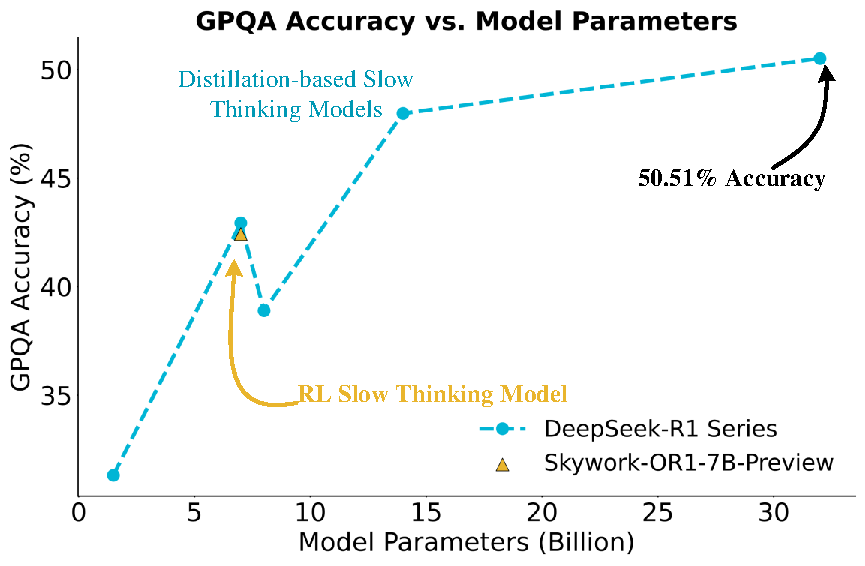
\includegraphics[width=\columnwidth]{images/slow-thinking.pdf}
%     % \vspace{-2ex}
%     \caption{Accuracy of the slow thinking model on the GPQA dataset.}
%     \vspace{-3ex}
%     \label{slow-thinking-gpqa}
% \end{figure}





